%%%%%%%%%%%%%%%%%%%%%%%%%%%%%%%%%%%%%%%%%%%%%%%%
%
%  CHAPTER 4: Implementation and Results
%
%%%%%%%%%%%%%%%%%%%%%%%%%%%%%%%%%%%%%%%%%%%%%%%%

\newcommand{\twosub}[2]{\begin{subarray}{l}{#1}\\{#2}\end{subarray}}

%%%%%%%%%%%%%%%%%%%%%%%%%%%%%%%%%%%%%%%%%%%%%%%%
% Section 4.1 - Introduction
%%%%%%%%%%%%%%%%%%%%%%%%%%%%%%%%%%%%%%%%%%%%%%%%
% \section{Introduction}\label{sec:Introduction}

As discussed in Chapter \ref{ch:ADCs and DSMs}, \DS modulators use oversampling and
feedback to attenuate
inband quantization noise power. Because many discrete-time \DS modulators can be modeled
by the LTI system shown in Figure \ref{fig:linear_simulation_model_2}, the NTF and STF can
be described by \eqref{eq:NTF}
and \eqref{eq:STF}.
 %-----------------------
\begin{figure}[htbp]
	\centering
	\includegraphics{./final_figures/linear_block_simulation.eps}
	\caption{$\Delta\Sigma$ Modulator Linear Model Block Diagram}
	\label{fig:linear_simulation_model_2}
\end{figure}
%-----------------------
As such, the NTF and STF represent discrete recursive filters, which are often designed
using digital IIR filter design techniques. The structure of a \DS modulator dictates
that the STF and NTF share a common set of poles. As such, the design of either the STF 
or NTF has implications for the design of the other. Because a \DS modulator's performance
depends mostly on the shape of the inband NTF, the NTF is typically designed first. The
zeros of the STF are then designed to accommodate the poles that result from the preceding
NTF design.

NTFs are often designed using traditional filters, such as Butterworth
and Chebyshev filters \cite{valkenburg_analog_1995}. These methods result in optimal
designs for certain performance criterion, often without consideration for others. For
example, a \DS modulator's NTF that has been designed using a Chebyshev filter is optimal
for dynamic range performance but not necessarily optimal for SNR performance.
Traditional filters such as Chebyshev filters generate NTFs with well defined passbands
which are not required for most NTFs. Also, these methods are not always easily adaptable
to the frequency response specifications required by \DS modulators for certain
applications \cite{IASTED_greg}.

Other contemporary methods often use numerical methods to determine optimal NTFs. For
example, the Delta Sigma Toolbox available for MATLAB\textsuperscript{\textregistered}
generates \DS modulator NTFs by determining NTF zeroes which minimize the
inband quantization noise power\cite{schreier_understanding_2004}. This technique
determines these optimized zeroes by setting the first derivative of the inband power
spectral density to zero and solving the resulting equations.  After determining the
optimized zeroes, the NTF's poles are optimized using an iterative approach. Because
poles and zeros do not affect system functions independently and because this
technique determines the NTF's zeros independently from its poles, this
technique does not necessarily generate optimal designs. As such, it will be shown that
this method offers only marginal improvement with respect to SNR over traditional
polynomial based methods.

In this thesis, the Hybrid Orthogonal Genetic (HOG) algorithm, developed in Chapter 3, is
used to determine optimal NTFs and STFs. The overall design methodology is illustrated in
Figure \ref{fig:HOG_DSM_flow}. Specifically, this implementation of the HOG algorithm
evolves optimal NTFs by maximizing a weighted combination of inband SNR and DR. After
determining an optimal NTF, the HOG algorithm then evolves an optimal STF by minimizing
 the passband magnitude error and attenuating out of band signal energy. The resulting
NTFs and STFs are then rigorously simulated and analyzed to ensure stability and
performance\cite{stubberud_hybrid_2008}.
%-----------------------
\begin{figure}[htbp]
	\centering
	\includegraphics[height=0.65\textheight]{./final_figures/HOGA_DSM_flow.eps}
	\caption{Optimal \DS Modulator Design Flowchart}
	\label{fig:HOG_DSM_flow}
\end{figure}
%-----------------------

%%%%%%%%%%%%%%%%%%%%%%%%%%%%%%%%%%%%%%%%%%%%%%%%
% Section 4.2 - Objective Functions
%%%%%%%%%%%%%%%%%%%%%%%%%%%%%%%%%%%%%%%%%%%%%%%%
\section[Delta Sigma Modulator Design Objective Functions]
{$\Delta\Sigma$ Modulator Design Objective Functions}
\label{sec:DSM Design Objective Functions}
For this thesis, optimal NTFs and STFs are determined by approximating the NTF and STF
system functions so that the \DS modulator's SNR and DR are maximized. That is, cost
functions are minimized with respect to the NTF and STF coefficients such that the
effective resolution of the \DS modulator is maximized.

\subsection{NTF Objective Function}\label{sec:NTF_Objective_Function}
Ideally, a NTF magnitude response, $\lvert H(e^{j\omega})\rvert$,
would remove all signal energy in the stopband which implies that
%---------------------
\begin{equation}\label{eq:ideal_H_sb}
 \lvert H(e^{j\omega})\rvert=0,\qquad\omega\in\omega_\text{sb}
\end{equation}
%---------------------
where $\omega_\text{sb}$ is the set of stopband frequencies. For a lowpass \DS modulator,
$\omega_\text{sb}$, can be defined such that
$\omega_\text{sb}\in\{\omega:\lvert\omega\rvert\leq\omega_s\}$ for the stopband corner
frequency, $\omega_s$. However, to prevent the NTF from having all zero coefficients the
NTF's passband is ideally 1. Therefore, the ideal NTF magnitude response can be written as
%---------------------
\begin{equation}\label{eq:ideal_H_equation}
 \lvert H(e^{j\omega})\rvert=
\begin{cases}
0,& \omega\in\omega_\text{sb}\\
1,& \omega\in\omega_\text{pb}\\
\end{cases}
\end{equation}
%---------------------
where $\omega_\text{pb}$ is the set of passband frequencies. For a lowpass \DS modulator,
$\omega_\text{pb}$ can be defined such that
$\omega_\text{pb}\in\{\omega:\omega_p\leq\lvert\omega\rvert\leq\pi\}$ for the
passband corner frequency, $\omega_p$.
 
In practice, the ideal frequency response in \eqref{eq:ideal_H_equation} cannot be
achieved, and therefore, $\lvert H(e^{j\omega})\rvert$ must be approximated. As such, the
difference between the ideal magnitude response and the realized NTF magnitude response,
$\lvert\NTF(e^{j\omega})\rvert$, is referred to as the NTF magnitude response
error, $\lvert H_e(e^{j\omega})\rvert$; that is,
%---------------------
\begin{equation}\label{eq:H_error_mag}
 \lvert H_e(e^{j\omega})\rvert = \lvert
H(e^{j\omega})\rvert-\lvert\NTF(e^{j\omega})\rvert.
\end{equation}
%---------------------
Substituting \eqref{eq:ideal_H_equation} into \eqref{eq:H_error_mag}, it can be seen
that for a lowpass \DS modulator
%---------------------
\begin{equation}\label{eq:H_error_mag_2}
 \lvert H_e(e^{j\omega})\rvert=
\begin{cases}
\lvert \NTF(e^{j\omega})\rvert,& \omega\in\omega_\text{sb}\\
 1- \lvert\NTF(e^{j\omega})\rvert,& \omega\in\omega_\text{pb}
\end{cases}.
\end{equation}
%---------------------

\subsubsection{SNR Optimization}
To maximize the SNR over the NTF's stopband, the noise power in the NTF's stopband must be
minimized. As demonstrated by \eqref{eq:LTI_average_output_power} in Chapter \ref{ch:ADCs
and DSMs}, a \DS modulator's output quantization noise power, $P_q$, over the stopband can
be written as
%---------------------
\begin{equation}\label{eq:output_power_psd}
P_q=\frac{1}{2\pi}\int_{\omega\in\omega_\text{sb}}\lvert
\NTF(e^{j\omega})\rvert^2\bm{S}_e(e^{j\omega})d\omega
\end{equation}
%---------------------
where $\bm{S}_e(e^{j\omega})$ is the power spectral density of the quantization noise. As
shown in \eqref{eq:quantization_noise_psd_6},
$$\bm{S}_{e(n)}(e^{j\omega})=\frac{\Delta^2}{12}$$ which implies that
%---------------------
\begin{equation}\label{eq:output_noise_power}
P_q=\frac{\Delta^2}{12}\left(\frac{1}{2\pi}\right)\int_{\omega\in\omega_\text { sb } }
\lvert \NTF(e^{j\omega})\rvert^2 d\omega.
\end{equation}
%---------------------
Because the $p$-norm, denoted $\lVert\cdot\rVert_p$, of a continuous-time signal,
$x(t)$, is defined as
%---------------------
\begin{equation}\label{eq:p_norm}
\lVert x(t)\rVert_p=\left(\int_{t\in T}\lvert x(t)\rvert^p dt\right)^\frac{1}{p}
\end{equation}
%---------------------
where $T$ denotes some fixed time interval, $P_q$ can be written as
%---------------------
\begin{equation}\label{eq:parseval_3}
P_q=
\frac{\Delta^2}{12}\left(\frac{1}{2\pi}\right)\int_{\omega\in\omega_\text { sb } }
\lvert \NTF(e^{j\omega})\rvert^2 d\omega=
\frac{\Delta^2}{12}\left(\frac{1}{2\pi}\right)\lVert
\NTF(e^{j\omega})\rVert^2_{\twosub{2}{\omega\in\omega_\text{sb}}}.
\end{equation}
%---------------------
Therefore, a \DS modulator's SNR can be maximized by minimizing $\lVert
\NTF(e^{j\omega})\rVert^2_{\twosub{2}{\omega\in\omega_\text{sb}}}$.

\subsubsection{DR Optimization}
Recall that DR is defined as the ratio of the maximum to the minimum detectable
signal levels. As such, the DR can be maximized my minimizing the largest noise
component over the stopband of the NTF. Because the $\infty$-norm of a
continuous-time signal, $x(t)$, can be written as
%---------------------
\begin{equation}\label{eq:inf_norm}
\lVert x(t)\rVert_\infty=\lim_{p\to\infty}\left(\int_{t\in T}\lvert x(t)\rvert^p
dt\right)^\frac{1}{p}=\max\langle\lvert x(t)\rvert\rangle.
\end{equation}
%---------------------
Therefore, a \DS modulator's DR can be maximized by minimizing $\lVert
\NTF(e^{j\omega})\rVert_{\twosub{\infty}{\omega\in\omega_\text{sb}}}$.

\subsubsection{Passband Optimization}
It has been observed that the likelihood of \DS modulator stability can be increased by
designing NTFs that have approximately unity gain at $\pi$ radians/sample and that
 do not have passband peaking\cite{schreier_empirical_1993}. As such, minimizing the
1-norm of the magnitude error over the passband, $\lVert
1-\vert\NTF(e^{j\omega})\rvert\rVert_{\twosub{1}{\omega\in\omega_\text{pb}}}$, can
produce passband magnitude responses with approximately unity gain at $\pi$
radians/sample and that do not have passband peaking.

\subsubsection{Stability}
Because the NTF is modeled as discrete-time LTI systems, its pole locations,
$\left\{\gamma_k\right\}$, must lie within the unit circle to realize a stable system;
that is, for the \DS modulator to be stable, 
%---------------------
\begin{equation}\label{eq:stability}
\lvert \gamma_k \rvert < 1.
\end{equation}
%---------------------
As such, the solution space for the approximated NTF must be constrained such that none of
its poles lie outside the unit circle.

\subsubsection{Cost Function}
The NTF cost function is the weighted sum of the approximated magnitude response errors
and can be written as
%---------------------
\begin{equation}\label{eq:NTF_cost_function}
J_{\NTF}=
\alpha\lVert\NTF(e^{j\omega})\rVert^2_{\twosub{2}{\omega\in\omega_\text{sb}}}+
\beta\lVert\NTF(e^{j\omega})\rVert_{\twosub{\infty}{\omega\in\omega_\text{sb}}}+
\left(1-\alpha-\beta\right)\lVert 1-\lvert\NTF(e^{j\omega})\rvert\rVert_{\twosub{1}{
\omega\in\omega_\text{pb}}}
\end{equation}
%---------------------
where $\alpha$ and $\beta$ are weighting coefficients such that
$\left\{\alpha,\beta\right\}\geq0$ and $\alpha+\beta\leq1$, $\norm{\cdot}_p$ denotes the
$p$-norm, and all the pole locations are constrained such that they lie within the unit
circle.

As discussed in Chapter \ref{ch:ADCs and DSMs}, NTFs are typically modeled as LTI
systems that can be described by rational functions. Because minimizing the $p$-norm of a
rational function is a difficult analytical problem, the cost function is minimized
numerically. Thus, the NTF is approximated by calculating the DFT over the stopband and
the passband.

For example, the $N_s$-point DFT of the NTF can be written as
%---------------------
\begin{equation}\label{eq:sampling_frequency_response}
\NTF(k)=\NTF(e^{j\omega})\Bigr\rvert_{\omega=\frac{2\pi}{N_s}k}
\end{equation}
%---------------------
for $k\in\{I:0\leq k\leq N_s-1\}$. Thus,
%---------------------
\begin{equation}\label{eq:sampling_frequency_response_2}
\lVert\NTF(e^{j\omega})\rVert^2_{\twosub{2}{\omega\in\omega_\text{sb}}}
\approx
\quad\rVert\NTF(k)\rVert^2_{\twosub{2}{k\in k_\text{sb}}}
\end{equation}
%---------------------
where $k_\text{sb}\in\{k:0\leq k\leq N_s-1$ and
$\frac{2\pi}{N_s}k\in\omega_\text{sb}\}$ and where the $p$-norm of a discrete signal,
$x(n)$, is defined as
%---------------------
\begin{equation}\label{eq:vector_p_norm}
\lVert x(n)\rVert_p=\left(\sum_{k=1}^{N}\lvert x(k)\rvert^p\right)^\frac{1}{p}
\end{equation}
%---------------------
for a signal of length $N$. As such, the SNR can be maximized by minimizing the
2-norm squared of the approximated stopband frequency response,
$\lVert\NTF(k)\rVert^2_{\twosub{2}{k\in k_\text{sb}}}$, where
$k_\text{sb}=\left\{k:\frac{2\pi}{N_s}k\in\omega_\text{sb}\right\}.$ It can also be seen
that 
%---------------------
\begin{equation}\label{eq:vector_inf_norm_cont_equal}
\lVert\NTF(e^{j\omega})\rVert_{\twosub{\infty}{\omega\in\omega_\text{sb}}}
\approx
\quad\rVert\NTF(k)\rVert_{\twosub{\infty}{k\in k_\text{sb}}}
\end{equation}
%---------------------
where the $\infty$-norm of a discrete signal, $x(n)$, is defined as 
%---------------------
\begin{equation}\label{eq:vector_inf_norm}
\lVert x(n)\rVert_\infty=\lim_{p\to\infty}\left(\sum_{k=1}^{N}\lvert x(k)\rvert^p
\right)^\frac{1}{p}=\max\langle\lvert x(k)\rvert\rangle.
\end{equation}
%---------------------
for a signal of length $N$. As such, the DR can be maximized by minimizing the
$\infty$-norm of the approximated stopband frequency response,
$\lVert\NTF(k)\rVert_{\twosub{\infty}{k\in k_\text{sb}}}$, for
$$k_\text{sb}=\left\{k:\frac{2\pi}{N_s}k\in\omega_\text{sb}\right\}.$$

Similarly, the $N_p$-point DFT of the NTF can be written as 
%---------------------
\begin{equation}\label{eq:sampling_frequency_response_pb}
\NTF(k)=\NTF(e^{j\omega})\Bigr\rvert_{\omega=\frac{2\pi}{N_p}k}
\end{equation}
%---------------------
for $k\in\{I:0\leq k\leq N_p-1\}$. Thus,
%---------------------
\begin{equation}\label{eq:sampling_frequency_response_2_pb}
\lVert\NTF(e^{j\omega})\rVert_{\twosub{1}{\omega\in\omega_\text{pb}}}
\approx
\quad\rVert\NTF(k)\rVert_{\twosub{1}{k\in k_\text{pb}}}
\end{equation}
%---------------------
where $k_\text{pb}=\{k:0\leq k\leq N_p-1\text{ and
}\frac{2\pi}{N_p}k\in\omega_\text{pb}\}$. As such, the shape of the passband magnitude
response can be determined by minimizing the 1-norm of the approximated passband magnitude
error response, $\lVert1-\lvert\NTF(k)\rvert\rVert_{\twosub{1}{k\in k_\text{pb}}}$, for
$k_\text{pb}=\left\{k:\frac{2\pi}{N_p}k\in\omega_\text{pb}\right\}.$

Therefore, the NTF's objective function, $J_{\NTF}$, in \eqref{eq:NTF_cost_function} can
be approximated as 
%-----------------------
\begin{equation}\label{eq:NTF_objective_function}
J_{\NTF}=\\
\alpha\norm{\NTF(k)}^2_{\twosub{2}{k\in k_\text{sb}}}
+\beta\norm{\NTF(k)}_{\twosub{\infty}{k\in k_\text{sb}}}
+(1-\alpha-\beta)\norm{1-\lvert\NTF(k)\rvert}_{\twosub{1}{k\in k_\text{pb}}}
\end{equation}
%-----------------------
where $\left\{\alpha,\beta\right\}\geq0$ and $\alpha+\beta\leq1$ and all the pole
locations are constrained such that they lie within the unit circle. For this thesis,
optimal NTFs were designed with $\alpha=\beta=0.25$.

For example, the cost function illustrated in Figure \ref{fig:NTF_obj_fn} can be
minimized to determine a highpass NTF for a lowpass \DS modulator which is optimal
with respect to a weighted combination of SNR and DR.
%-----------------------
\begin{figure}[htbp]
	\centering
	\includegraphics*[clip,width=\textwidth,viewport=0 0 475
175]{./final_figures/NTF_objective_fn.eps}
	\caption{NTF Magnitude Response Objective Function}
	\label{fig:NTF_obj_fn}
\end{figure}
%-----------------------

\subsection{STF Objective Function}\label{sec:STF_Objective_Function}
Ideally, a STF magnitude response, $\lvert H(e^{j\omega})\rvert$,
would remove all signal energy in the stopband and the passband would be one; that is, an
ideal STF magnitude response, $\lvert H(e^{j\omega})\rvert$, can be written as
%---------------------
\begin{equation}\label{eq:ideal_H_equation_STF}
\lvert H(e^{j\omega})\rvert=
\begin{cases}
0,& \omega\in\omega_\text{sb}\\
1,& \omega\in\omega_\text{pb}\\
\end{cases}
\end{equation}
%---------------------
where $\omega_\text{sb}$ is the set of stopband frequencies and $\omega_\text{pb}$ is the
set of passband frequencies. In practice, the ideal frequency response in
\eqref{eq:ideal_H_equation_STF} cannot be achieved, and therefore, $\lvert
H(e^{j\omega})\rvert$ must be approximated. As such, the difference between the ideal
magnitude response and the realized STF magnitude response, $\lvert
\STF(e^{j\omega})\rvert$, is referred to as the STF magnitude response
error, $H_e(e^{j\omega})$; that is,
%---------------------
\begin{equation}\label{eq:H_error_mag_STF}
 H_e(e^{j\omega})= \lvert H(e^{j\omega})\rvert-\lvert\STF(e^{j\omega})\rvert.
\end{equation}
%---------------------
Comparing \eqref{eq:ideal_H_equation_STF} and \eqref{eq:H_error_mag_STF}, it can be seen
that for a lowpass \DS modulator
%---------------------
\begin{equation}\label{eq:H_error_mag_2_STF}
\lvert H_e(e^{j\omega})\rvert=
\begin{cases}
\lvert \STF(e^{j\omega})\rvert,& \omega\in\omega_\text{sb}\\
 1- \lvert\STF(e^{j\omega})\rvert,& \omega\in\omega_\text{pb}
\end{cases}
\end{equation}
%---------------------

\subsubsection{STF Optimization}
Recall that the stopband signal energy can be minimized by minimizing the 2-norm squared
of the frequency response, $\lVert \STF(e^{j\omega})\rVert^2_2$, for $\omega
\in\omega_\text{sb}$. Similarly, minimizing the 1-norm of the passband magnitude error,
$\lVert 1- \lvert\STF(e^{j\omega})\rvert\rVert_1$, for $\omega\in\omega_\text{pb}$
produces magnitude responses which are approximately unity gain and without
passband peaking.

\subsubsection{Cost Function}
Therefore, the STF cost function, which is the weighted sum of the
approximated magnitude response errors, can be written as
%---------------------
\begin{equation}\label{eq:STF_cost_function}
J_{\STF}=
\zeta\lVert\STF(e^{j\omega})\rVert^2_{\twosub{2}{\omega\in\omega_\text{sb}}}+
\left(1-\zeta\right)\lVert 1-\lvert\STF(e^{j\omega})\rvert\rVert_{\twosub{1}{
\omega\in\omega_\text{pb}}}
\end{equation}
%---------------------
where $\zeta$ is a weighting coefficients such that $0\leq\zeta\leq1$ and $\norm{\cdot}_p$
denotes the $p$-norm.

However, as discussed in Chapter \ref{ch:ADCs and DSMs}, STFs are typically modeled as LTI
systems that can be described by rational functions. Because minimizing the $p$-norm of a
rational function is a difficult analytical problem, the cost function is minimized
numerically. Thus, the STF is approximated by calculating the DFT over the stopband and
the passband.

As was done for the NTF, an $N_s$-point DFT and a $N_p$-point DFT can be used to
approximate the cost function given in \eqref{eq:STF_cost_function} such that 
%-----------------------
\begin{equation}\label{eq:STF_objective_function}
J_{\STF}=
\zeta\norm{\STF(k)}^2_{\twosub{2}{k\in k_\text{sb}}}
+(1-\zeta)\norm{1-\lvert\STF(k)\rvert}_{\twosub{1}{k\in k_\text{pb}}}
\end{equation}
%-----------------------
where $0\leq\zeta\leq1$. For this thesis, optimal STFs were designed with a weighting
coefficient of $\zeta=0.5$.

For example, the cost function illustrated in Figure \ref{fig:STF_obj_fn} can be
minimized to determine an optimal STF for a lowpass \DS modulator.
%-----------------------
\begin{figure}[htbp]
	\centering
	\includegraphics*[clip,width=\textwidth,viewport=0 0 475
175]{./final_figures/STF_objective_fn.eps}
	\caption{STF Magnitude Response Objective Function}
	\label{fig:STF_obj_fn}
\end{figure}
%-----------------------

\subsection{Objective Function Minimization}
The cost functions shown in \eqref{eq:NTF_objective_function} and
\eqref{eq:STF_objective_function} are known to be highly multimodal and non-differentiable
equations\cite{rabiner_linear_1974}. As such, the HOG algorithm presented in Chapter
\ref{ch:Optimization and Genetic Algorithms} has been implemented as a constrained global
optimizer to minimize the cost functions thereby producing \DS modulator system functions
which are optimal with respect to their cost functions.

The HOG algorithm constrains the solution space through penalization. For example, a large
penalty value is returned if any of the evolved poles fall outside the unit circle. In
addition, the general shape of the magnitude response is constrained such that proposed
filter solutions which do not conform to the desired magnitude response shape (e.g.
highpass or lowpass) are penalized. For example, the NTF magnitude response evaluated at
DC must be sufficiently low or a large penalty value is returned. Similarly, the STF
magnitude response evaluated at $\pi$ radians/sample must be sufficiently low or a large
penalty value is returned. In general, penalties are selected so that they do  not
restrict the solution space any more than necessary which has been shown to result in
sub-optimal solutions \cite{karaboga_design_2004}.

%%%%%%%%%%%%%%%%%%%%%%%%%%%%%%%%%%%%%%%%%%%%%%%%
% Section 4.2 - HOG Algorithm Implementation
%%%%%%%%%%%%%%%%%%%%%%%%%%%%%%%%%%%%%%%%%%%%%%%%
\section{HOG Algorithm Implementation}\label{sec:HOG Algorithm Implementation}
For this thesis, the HOG algorithm, developed in Chapter \ref{ch:Optimization and Genetic
Algorithms}, is used to evolve a population
of chromosomes which contain the polynomial coefficients for the rational functions which
represent the NTF and STF. Once the population has been initialized to the regions
surrounding the solutions of traditional polynomials (e.g the Chebyshev polynomial), the
HOG algorithm iteratively evolves better polynomial coefficients until the population
converges to the optimum. For this implementation, the optimal polynomial coefficients are
determined by minimizing the cost functions in \eqref{eq:NTF_objective_function} and
\eqref{eq:STF_objective_function} thereby producing system functions which are optimal
with respect to SNR and DR.

%%%%%%%%%%%%%%%%%%%%%%%%%%%%%%%%%%%%%%%%%%%%%%%%
% Section 4.2.2 - Chromosome and Population Structure
%%%%%%%%%%%%%%%%%%%%%%%%%%%%%%%%%%%%%%%%%%%%%%%%
\subsection{Chromosome and Population Structure}\label{sec:Chromosome and Population
Structure}
Recall that structurally, chromosomes are implemented as arrays of length $K$. As such,
these arrays are populated with $K$ alleles, that are iteratively modified
during the evolutionary process. For filter design applications, the alleles can
correspond to the polynomial coefficients of the NTF or STF which have the general form
%---------------------
\begin{equation}\label{eq:chromosome_NTF_polynomial}
H(z)=\frac{\displaystyle\sum_{n=0}^{N}{a_n
z^{-n}}}{\displaystyle\sum_{n=0}^{N}{b_n z^{-n}}}
\end{equation}
%---------------------
where $\{a_{n}\}$ and $\{b_{n}\}$ are the sets of real polynomial coefficients and $N$ is
the order of the filter. However, populating the chromosomes directly with the polynomial
coefficients,
$\{a_n\}$ and $\{b_n\}$, yields chromosomes which are very sensitive to perturbation
during the evolutionary process. To reduce coefficient sensitivity,
\eqref{eq:chromosome_NTF_polynomial} can be written in its zero-pole-gain form,
%---------------------
\begin{equation}\label{eq:chromosome_NTF_pole_zero}
H(z)=\psi\cdot\frac{\displaystyle\prod_{n=1}^{N}{\bigl(1-c_n z^{-1}\bigr)}}
{\displaystyle\prod_{n=1}^{N}{\bigl(1-d_n z^{-1}\bigr)}}
\end{equation}
%---------------------
where $\{c_n\}$ is the set containing the system function's zeros, $\{d_n\}$ is the set
containing the system function's poles, and $\psi$ represents the system function's gain.
The alleles then correspond to the system function's zeros, poles, and gain. However, for
filters with real coefficients, these algorithms must explicitly manage complex conjugate
pairs of poles and zeros which can significantly lengthen run times. To reduce coefficient
sensitivity and simplify the management of complex conjugate pairs of poles and zeros, the
chromosomes are structured specifically so that the system function, $H(z)$, has the form
%---------------------
\begin{equation}\label{eq:chromosome_NTF}
H(z)=\psi\biggl(\frac{1-a_1 z^{-1}}{1-b_1 z^{-1}}\biggr)^m
\displaystyle\prod_{n=1}^{M}\frac{\bigl(1+c_{1n}z^{-1}+c_{2n}z^{-2}\bigr)}{\bigl(1+d_{1n}
z^{-1}+d_{2n}z^{-2}\bigr)}
\end{equation}
%---------------------
where $M$ is the number of second-order-sections, $\psi$ represents the system
function's gain, and $m$ is 1 or 0 for odd or even ordered systems,
respectively\cite{kit-sang_tang_design_1998}.
 
For this thesis, the NTF is equivalent to \eqref{eq:chromosome_NTF}; that
is
%---------------------
\begin{equation}\label{eq:NTF_system_function}
\NTF(z)=\psi_N\biggl(\frac{1-a_1 z^{-1}}{1-b_1 z^{-1}}\biggr)^m
\displaystyle\prod_{n=1}^{M}\frac{\bigl(1+c_{1n}z^{-1}+c_{2n}z^{-2}\bigr)}{\bigl(1+d_{1n}
z^{-1}+d_{2n}z^{-2}\bigr)}\text{.}
\end{equation}
%---------------------
Thus, for a NTF described by \eqref{eq:NTF_system_function},
the structural chromosome array, $\mathcal{C}_{\text{NTF}}$, of length, $K_N$, where
%---------------------
\begin{equation}\label{eq:NTF_chromosome_length}
 K_N=4M+2m+1,
\end{equation}
%---------------------
can be written as
%---------------------
\begin{equation}\label{eq:chromosome_array_even}
\mathcal{C}_{\text{NTF}}=\left[c_{11},c_{12},d_{11},d_{12},c_{21},c_{22},d_{21},d_{
22},\dotsc,c_{M1},c_{M2},d_{M1},d_{M2},\psi_N\right]^T
\end{equation}
%---------------------
for even ordered systems and
%---------------------
\begin{equation}\label{eq:chrmosome_array_odd}
\mathcal{C}_{\text{NTF}} =
\left[a_1,b_1,c_{11},c_{12},d_{11},d_{12},c_{21},c_{22},d_{ 21},
d_{22},\dotsc,c_{M1},c_{M2},d_{M1},d_{M2},\psi_N\right]^T
\end{equation}
%---------------------
for odd ordered systems where the superscript $T$ denotes the transpose operator. As such,
for a NTF of order $2M+1$, a population, $\mathbb{G}_{\text{NTF}}$, of $n$ chromosomes can
be written as
%---------------------
\begin{equation}\label{eq:population}
\mathbb{G}_{\text{NTF}}
=\Bigl[\mathcal{C}_{\text{NTF},1}\dashline\mathcal{C}_{\text{NTF},2}
\dashline\dotsb\dashline\mathcal{C}_{\text{NTF},n}\Bigr]=
\begin{pmatrix}
a_{1,1}&  a_{1,2}& \hdotsfor{1}& a_{1,n-1}& a_{1,n} \\
b_{1,1}&  b_{1,2}& \hdotsfor{1}& b_{1,n-1}& b_{1,n} \\
c_{11,1}&  c_{11,2}& \hdotsfor{1}& c_{11,n-1}& c_{11,n} \\
c_{12,1}&  c_{12,2}& \hdotsfor{1}& c_{12,n-1}& c_{12,n} \\
d_{11,1}&  d_{11,2}& \hdotsfor{1}& d_{11,n-1}& d_{11,n} \\
d_{12,1}& d_{12,2}& \hdotsfor{1}& d_{12,n-1}& d_{12,n} \\
\vdots&\vdots&\ddots&\vdots&\vdots\\
c_{M1,1}& c_{M1,2}&\hdotsfor{1}& c_{M1,n-1}& c_{M1,n} \\
c_{M2,1}& c_{M2,2}&\hdotsfor{1}& c_{M2,n-1}& c_{M2,n} \\
d_{M1,1}& d_{M1,2}&\hdotsfor{1}& d_{M1,n-1}& d_{M1,n} \\
d_{M2,1}& d_{M2,2}&\hdotsfor{1}& d_{M2,n-1}& d_{M2,n} \\
\psi_{N,1}& \psi_{N,2}&\hdotsfor{1}& \psi_{N,n-1}& \psi_{N,n} \\	
\end{pmatrix}
\end{equation}
%-----------------------
where $\mathbb{G}_{\text{NTF}}$ is a $K_N\times n$ matrix and $\mathcal{C}_{\text{NTF},n}$
is the $n$th chromosome. 

Because NTFs and STFs share a common set of poles and the NTF is designed first, the STF
system function can be written as
%---------------------
\begin{equation}\label{eq:STF_system_function}
 \STF(z)=\psi_S\biggl(\frac{1-\rho_1 z^{-1}}{1-b_1 z^{-1}}\biggr)^m
\displaystyle\prod_{n=1}^{M}\frac{\bigl(1+\nu_{1n}z^{-1}+\nu_{2n}z^{-2}\bigr)}{\bigl(1+d_{
1n }z^{-1}+d_{2n}z^{-2}\bigr)}\text{.}
\end{equation}
%---------------------
Because the pole locations are established by the design of the NTF, only the STF's zero
locations are perturbated during the optimization process. As such, for a STF system
function described by \eqref{eq:STF_system_function},
the structural chromosome array, $\mathcal{C}_{\text{STF}}$, of length $K_S$, where
%---------------------
\begin{equation}\label{eq:STF_chromosome_length}
 K_S=2M+m+1,
\end{equation}
%---------------------
can be written as
%---------------------
\begin{equation}\label{eq:STF_chromosome_array_even}
\mathcal{C}_{\text{STF}}=\left[\nu_{11},\nu_{12},\nu_{21},\nu_{22},\dotsc,\nu_{M1},
\nu_{M2},\psi_S\right]^T
\end{equation}
%---------------------
for even ordered systems and
%---------------------
\begin{equation}\label{eq:STF_chrmosome_array_odd}
\mathcal{C}_{\text{STF}} =
\left[\rho_1,\nu_{11},\nu_{12},\nu_{21},\nu_{22},\dotsc,\nu_{M1},\nu_{M2},
\psi_S\right]^T
\end{equation}
%---------------------
for odd ordered systems. As such, for a STF of order $2M+1$, a population,
$\mathbb{G}_{\text{STF}}$, of $n$ chromosomes can be written as
%---------------------
\begin{equation}\label{eq:STF_population}
\mathbb{G}_{\text{STF}}
=\Bigl[\mathcal{C}_{\text{STF},1}\dashline\mathcal{C}_{\text{STF},2}
\dashline\dotsb\dashline\mathcal{C}_{\text{STF},n}\Bigr]=
\begin{pmatrix}
\rho_{1,1}&  \rho_{1,2}& \hdotsfor{1}& \rho_{1,n-1}& \rho_{1,n} \\
\nu_{11,1}&  \nu_{11,2}& \hdotsfor{1}& \nu_{11,n-1}& \nu_{11,n} \\
\nu_{12,1}&  \nu_{12,2}& \hdotsfor{1}& \nu_{12,n-1}& \nu_{12,n} \\
\vdots&\vdots&\ddots&\vdots&\vdots\\
\nu_{M1,1}& \nu_{M1,2}&\hdotsfor{1}& \nu_{M1,n-1}& \nu_{M1,n} \\
\nu_{M2,1}& \nu_{M2,2}&\hdotsfor{1}& \nu_{M2,n-1}& \nu_{M2,n} \\
\psi_{S,1}& \psi_{S,2}&\hdotsfor{1}& \psi_{S,n-1}& \psi_{S,n} \\	
\end{pmatrix}
\end{equation}
%-----------------------
where $\mathbb{G}_{\text{STF}}$ is a $K_S\times n$ matrix and
$\mathcal{C}_{\text{STF},n}$ is the $n$th chromosome. 

%%%%%%%%%%%%%%%%%%%%%%%%%%%%%%%%%%%%%%%%%%%%%%%%
% Section 4.2.3 - Algorithm Parameters
%%%%%%%%%%%%%%%%%%%%%%%%%%%%%%%%%%%%%%%%%%%%%%%%
\subsection{Algorithm Parameters}\label{sec:Algorithm Paramters}
The relative size of a population dictates the nature of the results. For example, large
unconstrained populations offer a broad evaluation of the performance surface at the
expense of convergence speed and steady-state misadjustment. Conversely, small
constrained populations converge quickly at the expense of increased population
variance. Further, selecting the appropriate size for a population is directly related
to the complexity, or dimensionality, of the problem space. However, the relationship
between problem space complexity and requisite population size is typically either poorly
defined or unknown \cite{alander_optimal_1992}. As such, for constrained problem spaces,
the most important concept is often minimum population size. However, because the minimum
population size is tightly coupled with the problem space complexity and therefore poorly
defined, it is typically refined or tuned a
posteriori\cite{alander_optimal_1992}\cite{schaffer_-_1989}. 

For this thesis, the initial size of the population has been restricted to 200; that is, 
to determine optimal NTFs and STFs, the HOG algorithm was initially configured with a
population size of 200 chromosomes. Because the poles of an IIR filter must
lie within the unit circle for the filter to be stable, the feasible solutions space
has been constrained such that each pole location, $\gamma$, lies within the unit circle
which implies that $$\lvert\gamma\rvert\leq1\text{.}$$ Because the interaction between
transfer function poles and zeros is implied in the desired magnitude response,
constraining the pole locations also indirectly constrains the zero locations. The
remaining HOG algorithm parameters are summarized in Table \ref{tbl:hog_dsm_setup}.
%----------------------------
\begin{table}[htbp]
 \begin{center}
 \caption[LP$\Delta\Sigma$M HOG Algorithm Parameters]{Low-Pass $\Delta\Sigma$ Modulator
Design: HOG Algorithm Parameters}
 \label{tbl:hog_dsm_setup}
 \begin{tabular}{ l c }\toprule
 \textbf{Description} & \textbf{Value} \\ \midrule
Problem Dimension & $K: K=K_N \text{or} K_S$ \\
Population Size & $200$ \\
Feasible Solution Space & $\lvert\gamma\rvert\leq1$ \\
Probability of Crossover & $P_c = 0.2$ \\
Probability of Mutation & $P_m = 0.02$ \\
Selection Pressure & $\eta^+ = 1.1$\\ \bottomrule
\end{tabular}
\end{center}
\end{table}

%%%%%%%%%%%%%%%%%%%%%%%%%%%%%%%%%%%%%%%%%%%%%%%%
% Section 4.2.4 - Population Initialization
%%%%%%%%%%%%%%%%%%%%%%%%%%%%%%%%%%%%%%%%%%%%%%%%
\subsection{Population Initialization}\label{sec:Population Initialization}
Although global optimization algorithms do not require a priori knowledge of
the performance surface to determine the optimum solution,  generalized constraints on
the objective function's solution space can greatly increase the speed of the algorithm's
convergence. Seeding the population with known solutions is often employed as a
test for conversion latency\cite{sarker_evolutionary_2002}. It has also been shown  that
seeding the population with solutions which are known to be near optimal can lead
to optimal solutions\cite{sarker_evolutionary_2002}.

Discrete-time \DS modulator NTFs which are designed using both contemporary and
traditional techniques have zeros which are distributed on or near segments of the unit
circle which correspond with the NTF's
stopband\cite{valkenburg_analog_1995}\cite{schreier_understanding_2004}.
Thus, it is plausible that the optimal zero locations will be distributed on or near
segments of the unit circle which correspond with the NTF's stopband as well. Further, if
it is assumed that the optimal zero locations are
distributed on or near the unit circle, then the optimal pole locations will likely be
proximal to the pole locations of both the traditional and contemporary NTF
filter designs.

Similarly, discrete-time \DS modulator STFs which are designed using traditional
techniques have zeroes which are distributed on or near the segments of the unit circle
corresponding to the STF's stopband. Thus, it is plausible that the optimal
zero locations will be distributed on or near segments of the unit circle which
correspond to the STF's stopband, as well. However, unlike the
NTF, which is designed first, the pole locations of the STF are fixed by the NTF design.
As such, it is assumed that the zero locations will be proximal to the zero locations for
traditional STF filter designs with pole locations determined by the optimal design of
the NTF.

Thus, the initial NTF and STF populations, $\mathbb{G}_{\NTF,0}$ and
$\mathbb{G}_{\STF,0}$, are seeded with chromosomes whose alleles are selected randomly
about the coefficients of a comparable NTF or STF, respectively. Specifically, their
respective chromosomes are determined by adding zero mean, standard normal random dither,
represented by $x$, with a fixed variance of 10\% (normalized with respect to the unit
circle) to the each of the Chebyshev polynomial coefficients where the system function is
described by \eqref{eq:chromosome_NTF} or \eqref{eq:STF_system_function}; that is, the
$k$th additive dither element, $\delta_k$, where $\bigl\{k\in I:1\leq k\leq
\left(K_N \;\text{or}\; K_S\right)\bigr\}$, can be expressed as 
%---------------------
\begin{equation}\label{eq:init_dither}
\delta_{k}=\frac{1}{\sqrt{0.2\pi}}e^{-\frac{x^2}{0.2}}
\end{equation}
%---------------------
for the random variable $x$.
 
Thus, the $n$th dithered chromosome,
$\tilde{\mathcal{C}}_{\NTF,n}$, belonging to an initial NTF population,
$\mathbb{G}_{\NTF,0}$, with a system function of order $2M+1$, can be written as 
%---------------------
\begin{equation}\label{eq:dithered_chromosome}
\begin{split}
&\tilde{\mathcal{C}}_{\NTF,n}= \\
&\bigl[
(a_{1}+\delta_{N,1}),(b_{1}+\delta_{N,2}),(c_{11}+\delta_{N,3}),(c_{12}+\delta_{N,4}),(d_
{ 11 }
+\delta_{N,5}),(d_{12}+\delta_{N,6}),\dotsc \\
&(c_{M1}+\delta_{N,K_N-4}),(c_{M2}+\delta_{N,K_N-3}),(d_{M1}+\delta_{N,K_N-2}),(d_{
M2 }
+\delta_{N,K_N-1}),(\psi_N+\delta_{N,K_N})\bigr]^T\\
&=\bigl[
\tilde{a}_1,\tilde{b}_1,\tilde{c}_{11},\tilde{c}_{12},\tilde{d}_{11},\tilde{d}_{12},
\tilde { c } _ { 21 } ,
\tilde{c}_{22},
\tilde{d}_{21},\tilde{d}_{22},\dotsc,\tilde{c}_{M1},\tilde{c}_{M2},\tilde{d}_{M1},
\tilde{d}_{M2},\tilde{\psi}_N\bigr]^T.
\end{split}
\end{equation}
%---------------------
where $\delta_{N,k}$ corresponds to the $k$th NTF additive dither element. Because a
population is defined as the aggregate of $n$ chromosomes, the initial
NTF population, $\mathbb{G}_{\NTF,0}$, can be written as
%---------------------
\begin{equation}
\mathbb{G}_{\NTF,0}
=\bigl[\tilde{\mathcal{C}}_{\NTF,1}\dashline\tilde{\mathcal{C}}_{\NTF,2}\dashline
\dotsb\dashline\tilde{\mathcal{C}}_{\NTF,n}\bigr]=
\begin{pmatrix}
\tilde{a}_{11,1}&\tilde{a}_{11,2}&\hdotsfor{1}&\tilde{a}_{11,n-1}&\tilde{a}_{11,n} \\
\tilde{b}_{12,1}&\tilde{b}_{12,2}&\hdotsfor{1}&\tilde{b}_{12,n-1}&\tilde{b}_{12,n} \\
\tilde{c}_{11,1}&\tilde{c}_{11,2}&\hdotsfor{1}&\tilde{c}_{11,n-1}&\tilde{c}_{11,n} \\
\tilde{c}_{12,1}&\tilde{c}_{12,2}&\hdotsfor{1}&\tilde{c}_{12,n-1}&\tilde{c}_{12,n} \\
\tilde{d}_{11,1}&\tilde{d}_{11,2}&\hdotsfor{1}&\tilde{d}_{11,n-1}&\tilde{d}_{11,n} \\
\tilde{d}_{12,1}&\tilde{d}_{12,2}&\hdotsfor{1}&\tilde{d}_{12,n-1}&\tilde{d}_{12,n} \\
\vdots&\vdots&\ddots&\vdots&\vdots						   \\
\tilde{c}_{M1,1}&\tilde{c}_{M1,2}&\hdotsfor{1}&\tilde{c}_{M1,n-1}&\tilde{c}_{M1,n} \\
\tilde{c}_{M2,1}&\tilde{c}_{M2,2}&\hdotsfor{1}&\tilde{c}_{M2,n-1}&\tilde{c}_{M2,n} \\
\tilde{d}_{M1,1}&\tilde{d}_{M1,2}&\hdotsfor{1}&\tilde{d}_{M1,n-1}&\tilde{d}_{M1,n} \\
\tilde{d}_{M2,1}&\tilde{d}_{M2,2}&\hdotsfor{1}&\tilde{d}_{M2,n-1}&\tilde{d}_{M2,n} \\
\tilde{\psi}_{N,1}&\tilde{\psi}_{N,2}&\hdotsfor{1}&\tilde{\psi}_{N,n-1}&\tilde{\psi}_{N,n
} \\
\end{pmatrix}
\end{equation}
where $\mathbb{G}_{\NTF,0}$ is a $K_N\times n$ matrix and $\tilde{\mathcal{C}}_{\NTF,k}$
is the $k$th dithered chromosome.

Similarly, the $n$th dithered chromosome, $\tilde{\mathcal{C}}_{\STF,n}$, belonging to an
initial STF population, $\mathbb{G}_{\STF,0}$, with a system function of order $2M+1$ can
be written as 
%---------------------
\begin{equation}\label{eq:dithered_chromosome_STF}
\begin{split}
\tilde{\mathcal{C}}_{\STF,n}=\bigl[
(\rho_{1}+\delta_{S,1}),(\nu_{11}+\delta_{S,2}),(\nu_{12}+\delta_{S,3}),\dotsc\\
 \dotsc,(\nu_{M1}+\delta_ { S,K_S-2 } ) ,
(\nu_{M2}+\delta_{S,K_S-1}),(\psi_S+\delta_{S,K_S})\bigr]^T\\
=\bigl[
\tilde{\rho_1},\tilde{\nu}_{11},\tilde{\nu}_{12},\tilde{\nu}_{21},\tilde{\nu}_{22},\dotsc,
\tilde{\nu}_{M1},\tilde{\nu}_{M2},\tilde{\psi}_S\bigr]^T
\end{split}
\end{equation}
%---------------------
where $\delta_{S,k}$ corresponds to the $k$th STF additive dither element. Because a
population is defined as the aggregate of $n$ chromosomes, the initial
STF population, $\mathbb{G}_{\STF,0}$, can be written as
%---------------------
\begin{equation}
\mathbb{G}_{\STF,0}
=\bigl[\tilde{\mathcal{C}}_{\STF,1}\dashline\tilde{\mathcal{C}}_{\STF,2}\dashline
\dotsb\dashline\tilde{\mathcal{C}}_{\STF,n}\bigr]=
\begin{pmatrix}
\tilde{\rho}_{11,1}&\tilde{\rho}_{11,2}&\hdotsfor{1}&\tilde{\rho}_{11,n-1}&\tilde{\rho}_{
11,n } \\
\tilde{\nu}_{11,1}&\tilde{\nu}_{11,2}&\hdotsfor{1}&\tilde{\nu}_{11,n-1}&\tilde{\nu}_{11,n}
\\
\tilde{\nu}_{12,1}&\tilde{\nu}_{12,2}&\hdotsfor{1}&\tilde{\nu}_{12,n-1}&\tilde{\nu}_{12,n}
\\
\vdots&\vdots&\ddots&\vdots&\vdots						   \\
\tilde{\nu}_{M1,1}&\tilde{\nu}_{M1,2}&\hdotsfor{1}&\tilde{\nu}_{M1,n-1}&\tilde{\nu}_{M1,n}
\\
\tilde{\nu}_{M2,1}&\tilde{\nu}_{M2,2}&\hdotsfor{1}&\tilde{\nu}_{M2,n-1}&\tilde{\nu}_{M2,n}
\\
\tilde{\psi}_{S,1}&\tilde{\psi}_{S,2}&\hdotsfor{1}&\tilde{\psi}_{S,n-1}&\tilde{\psi}_{S,n
} \\	
\end{pmatrix}
\end{equation}
where $\mathbb{G}_{\STF,0}$ is a $K_S\times n$ matrix and $\tilde{\mathcal{C}}_{\STF,k}$
is the $k$th dithered chromosome. 

%%%%%%%%%%%%%%%%%%%%%%%%%%%%%%%%%%%%%%%%%%%%%%%%
% Section 4.2.5 - Convergence
%%%%%%%%%%%%%%%%%%%%%%%%%%%%%%%%%%%%%%%%%%%%%%%%
\subsection{Convergence}\label{sec:Convergence}
Convergence during the evolution of a particular NTF or STF is defined as the lack of
further improvement over 100 successive generations following a minimum of 1000
generations. This criterion improves the probability that the evolved transfer functions
will be optimal with respect to their objective functions. However, this optimality does
not guarantee overall system stability; that is, even optimized NTFs and STFs may be
unstable when implemented in a $\Delta\Sigma$ modulator. Thus, overall design convergence
is achieved when the \DS modulator is stable and the observed DR and SNR are better than
the observations made for both traditional and contemporary $\Delta\Sigma$ modulator
designs of like order and OSR.

%%%%%%%%%%%%%%%%%%%%%%%%%%%%%%%%%%%%%%%%%%%%%%%%
% Section 4.3 - Simulation and Modeling
%%%%%%%%%%%%%%%%%%%%%%%%%%%%%%%%%%%%%%%%%%%%%%%%
\section{Simulation and Modeling}\label{sec:Simulation and Modeling}
Because SNR and DR are measures of an ADC's effective resolution and because SNR and DR
are measured in the frequency domain, the performance of a \DS modulator is characterized
by its observed output spectrum. While the linear quantizer model shown in Figure
\ref{fig:linear_quantizer_model} is sufficient for theoretical results and preliminary
system modeling, a simulation of the nonlinear system is necessary to determine the
realized effective resolution of a \DS modulator \cite{schreier_empirical_1993}. Thus, the
designed systems were verified using a simulator based on the block diagram shown in
Figure \ref{fig:linear_simulation_model_2}.

For this thesis, the output, $y(n)$, of a discrete-time \DS modulator is determined
using the linear difference equations which correspond to the blocks shown
in Figure \ref{fig:linear_simulation_model_2}. The \DS modulator's output is then
bandlimited to the Nyquist frequency of the input signal, $f_{\text{NQ}}$, where
$f_{\text{NQ}}\in\left[-f_s/2\text{OSR},f_s/2\text{OSR}\right]$, and then decimated by a
factor of $\text{OSR}/2$. Finally, the SNR and DR are calculated
using frequency domain analysis of the spectrum of the decimated output signal.

%%%%%%%%%%%%%%%%%%%%%%%%%%%%%%%%%%%%%%%%%%%%%%%%
% Section 4.3.1 - Linear Difference Equations
%%%%%%%%%%%%%%%%%%%%%%%%%%%%%%%%%%%%%%%%%%%%%%%%
\subsection{Linear Difference Equations}\label{sec:Linear Difference Equations}
Recall that the output, $y(n)$, of a \DS modulator as shown in Figure
\ref{fig:linear_simulation_model_2} can be expressed as 
%-----------------------
\begin{equation}\label{eq:general_form}
 Y(z) =\STF(z)X(z)+\NTF(z)E(z)
 \end{equation}
%-----------------------
where
%-----------------------
\begin{equation}\label{eq:STF_solution_1}
\STF(z)=\frac{F(z)G(z)}{1+z^{-1}G(z)H(z)}
\end{equation}
%-----------------------
and
%-----------------------
\begin{equation}\label{eq:NTF_solution_1}
\NTF(z)=\frac{1}{1+z^{-1}G(z)H(z)}\text{.}
\end{equation}
%-----------------------
Because STFs and NTFs are modeled as linear recursive filters, they can be written as
%-----------------------
\begin{equation}\label{eq:STF_poly_form}
\text{STF}(z)=\frac
{\displaystyle\sum_{k=0}^{N}{\alpha_k z^{-k}}}
{\displaystyle\sum_{k=0}^{N}{\beta_k  z^{-k}}}
\end{equation}
%-----------------------
and
%-----------------------
\begin{equation}\label{eq:NTF_poly_form}
\text{NTF}(z)=\frac
{\displaystyle\sum_{k=0}^{N}{\gamma_k z^{-k}}}
{\displaystyle\sum_{k=0}^{N}{\beta_k  z^{-k}}}
\end{equation}
%-----------------------
where $\{\alpha_k\}$, $\{\beta_k\}$, and $\{\gamma_k\}$ are the sets of real coefficients,
$\beta_0=1$, and
$N$ is the order of the numerator and denominator polynomials. 

\subsubsection{Canonical Solution}\label{sec:Canonical Solution}
Because $F(z)$, $G(z)$, and $H(z)$ are rational functions,
the STF and NTF can be expressed as
%-----------------------
\begin{equation}\label{eq:block_diagram_solving_STF}
\text{STF}(z) =\frac
{\left(\displaystyle\frac{F_n(z)}{F_d(z)}\displaystyle\frac{G_n(z)}{G_d(z)}\right)}
{1+z^{-1}\left(\displaystyle\frac{G_n(z)}{G_d(z)}\displaystyle\frac{H_n(z)}{
H_d(z) } \right)} 
 =\frac
{H_d(z)F_n(z)G_n(z)}
{F_d(z)\bigl(G_d(z)H_d(z)+z^{-1}G_n(z)H_n(z)\bigr)}
\end{equation}
%-----------------------
and
%-----------------------
\begin{equation}\label{eq:block_diagram_solving_NTF}
 \text{NTF}(z) = \frac
{1}
{1+z^{-1}\left(\displaystyle\frac{G_n(z)}{G_d(z)}\displaystyle\frac{H_n(z)}{
H_d(z) } \right)}  
 = \frac
{G_d(z)H_d(z)}
{G_d(z)H_d(z)+z^{-1}G_n(z)H_n(z)}\text{.}
\end{equation}
%-----------------------
Because of practical circuit implementation considerations, $F_d(z)$,$H_d(z)$, and
$G_n(z)$ are chosen so that $$F_d(z)=H_d(z)=G_n(z)=1\text{.}$$
Substituting $F_d(z)=H_d(z)=G_n(z)=1$ into \eqref{eq:block_diagram_solving_STF} and
\eqref{eq:block_diagram_solving_NTF},
%-----------------------
\begin{equation}\label{eq:block_equations_3_STF}
 \text{STF}(z) =\frac{F_{n}(z)}{G_{d}
(z)+z^{-1}H_{n} (z)}
\end{equation}
%-----------------------
and
%-----------------------
\begin{equation}\label{eq:block_equations_3_NTF}
 \text{NTF}(z) =\frac{G_{d}(z)}{G_{d}
(z)+z^{-1}H_{n} (z)}\text{.}
\end{equation}
%-----------------------
Comparing \eqref{eq:block_equations_3_STF} and \eqref{eq:block_equations_3_NTF} to
\eqref{eq:NTF_poly_form} and \eqref{eq:STF_poly_form}, it can be seen that 
%-----------------------
\begin{equation}\label{eq:block_diagram_to_canonical_Fn}
F_n(z)=\sum_{n=0}^{N}\alpha_n z^{-k},
\end{equation}
%-----------------------
%-----------------------
\begin{equation}\label{eq:block_diagram_to_canonical_Gd}
 G_d(z) =
\sum_{k=0}^{N}\gamma_k z^{-k},
\end{equation}
%-----------------------
and
%-----------------------
\begin{equation}\label{eq:block_diagram_to_canonical_num}
 G_d(z)+z^{-1}H_n(z) = \sum_{k=0}^{N}\beta_k z^{-k}.
\end{equation}
%-----------------------
Substituting \eqref{eq:block_diagram_to_canonical_Gd} into
\eqref{eq:block_diagram_to_canonical_num} and solving for $H_n(z)$
%-----------------------
\begin{equation}\label{eq:block_diagram_to_canonical_Hn}
 H_n(z) = \sum_{k=0}^{N}\left(\beta_k-\gamma_k\right)z^{-k+1}.
\end{equation}
%-----------------------
However, because $H_n(z)$ is causal, $\beta_0-\gamma_0=0$ which implies that
$\beta_0=\gamma_0=1$. Thus, $H_n(z)$ can be written as
%-----------------------
\begin{equation}\label{eq:block_diagram_to_canonical_Hn_2}
 H_n(z) = \sum_{k=1}^{N}\left(\beta_k-\gamma_k\right)z^{-k+1}.
\end{equation}
%-----------------------
Therefore, the LTI modeled subsystems, $F(z)$, $G(z)$, and $H(z)$, can be expressed as 
%-----------------------
\begin{equation}\label{eq:block_diagram_to_canonical_F}
F(z) = F_n(z)=\displaystyle\sum_{k=0}^{N}\alpha_k z^{-k},
\end{equation}
%-----------------------
%-----------------------
\begin{equation}\label{eq:block_diagram_to_canonical_G}
 G(z) = \frac{1}{G_d(z)} = \frac{1}{\displaystyle\sum_{k=0}^{N}\gamma_k
z^{-k}},
\end{equation}
%-----------------------
and
%-----------------------
\begin{equation}\label{eq:block_diagram_to_canonical_H}
 H(z) = H_n(z) =
\displaystyle\sum_{k=1}^{N}\left(\beta_k-\gamma_k\right)z^{-k+1}.
\end{equation}
%-----------------------

\subsubsection{Simulation Solution}\label{sec:Simulation Solution}
Replacing the linear noise model in Figure \ref{fig:linear_simulation_model_2} with a
nonlinear quantizer, the discrete-time \DS modulator in Figure
\ref{fig:linear_simulation_model_2} can be modeled as shown in Figure
\ref{fig:dsm_sim_model} where the quantizer's input is denoted as $Q_i(z)$.
%-----------------------
\begin{figure}[htbp]
 \centering
 \includegraphics{./final_figures/sim_block_diagram.eps}
 \caption{Discrete-Time Simulation Model}
 \label{fig:dsm_sim_model}
\end{figure}
%-----------------------
From observation of Figure \ref{fig:dsm_sim_model}, the quantizer's input, $Q_i(z)$, can
be
given as
%-----------------------
\begin{equation}\label{eq:quantizer_input_1}
Q_i(z) = G(z)\left(F(z)X(z)-z^{-1}H(z)Y(z)\right)\text{.}
\end{equation}
%-----------------------
Substituting \eqref{eq:block_diagram_to_canonical_F},
\eqref{eq:block_diagram_to_canonical_G}, and 
\eqref{eq:block_diagram_to_canonical_H} into \eqref{eq:quantizer_input_1}, the quantizer
input, $Q_i(z)$, can be expressed as
%-----------------------
\begin{equation}\label{eq:quantizer_input_2}
\begin{split}
 Q_i(z)&
=\left(\frac{F_n(z)}{G_d(z)}\right)X(z)-z^{-1}\left(\frac{H_n(z)}{G_d(z)}\right)Y(z)\\
 & = \left(\frac
{\displaystyle\sum_{k=0}^{N}\alpha_k z^{-k}}
{\displaystyle\sum_{k=0}^{N}\gamma_k z^{-k}}\right)X(z)
-z^{-1}\left(\frac
{\displaystyle\sum_{k=1}^{N}\left(\beta_k-\gamma_k\right)z^{-k}}
{\displaystyle\sum_{k=0}^{N} \gamma_k z^{-k}}\right)Y(z)\\
\end{split}
\end{equation}
%-----------------------
where $\gamma_0=1$. Alternatively, \eqref{eq:quantizer_input_2} can be written
such that
%-----------------------
\begin{equation}\label{eq:quantizer_input_3}
 Q_i(z)\left(\sum_{k=0}^{N} \gamma_k z^{-k}\right) =
\left(\displaystyle\sum_{k=0}^{N}\alpha_k z^{-k}\right)X(z)-
\left(\displaystyle\sum_{k=1}^{N}\left(\beta_k-\gamma_k\right)z^{-k}\right)Y(z)
\end{equation}
%-----------------------
where $\gamma_0=1$. Taking the inverse $z$-transform of
\eqref{eq:quantizer_input_3}, the quantizer
input, $q_i(n)$, can be written as
%-----------------------
\begin{equation}\label{eq:quantizer_input_discrete_time_1}
\sum_{k=0}^{N}\gamma_k q_i(n-k)=
\sum_{k=0}^{N}\alpha_k x(n-k) -
\sum_{k=1}^{N}\left(\beta_k-\gamma_k\right)y(n-k)
\end{equation}
%-----------------------
which implies that
%-----------------------
\begin{equation}\label{eq:quantizer_input_discrete_time_2}
q_i(n)=\sum_{k=0}^{N}\alpha_k x(n-k)-\sum_{k=1}^{N}\left(\beta_k-\gamma_k\right)y(n-k)-
\sum_{k=1}^{N}\gamma_k q_i(n-k).
\end{equation}
%-----------------------
Because a single-bit quantizer is implemented, the discrete-time output, $y(n)$, is
%-----------------------
\begin{equation}\label{eq:dt_dsm_output_discrete_time}
 y(n)=\mathop\text{sgn}\left[q_i(n)\right]
\end{equation}
%-----------------------
where $\mathop\text{sgn}[\cdot]$ is the signum function.

%%%%%%%%%%%%%%%%%%%%%%%%%%%%%%%%%%%%%%%%%%%%%%%%
% Section 4.3.2 - Decimation Filtering
%%%%%%%%%%%%%%%%%%%%%%%%%%%%%%%%%%%%%%%%%%%%%%%%
\subsection{Decimation Filtering}\label{sec:Decimation Filtering}
Consider a \DS modulator that has a sampling frequency, $f_s$,
and an OSR of $M$, which implies that $f_s=M 2f_0$. A \DS modulator's NTF filters the
quantization noise power, $P_{e(n)}$, over the quantizer's operational bandwidth,
$f_{\text{OS}}$, where $f_{\text{OS}}\in\left[-f_s/2,f_s/2\right]$. By bandlimiting the
ADC's digital output, $y(n)$,  to the input's signal's Nyquist frequency, $f_{\text{NY}}$,
where $f_{\text{NY}}\in\left[-f_0,f_0\right]$, the power spectral density of the input
signal is preserved while the quantization noise power contained in the output signal is
significantly decreased.

Ideally, the output signal would be bandlimited by an ideal digital lowpass filter,
referred to as a decimation filter, with a cutoff frequency of $f_s/2M$. However,
practical decimation filters require a finite transition bandwidth. As a 
result, quantization noise power from the transition band will alias into the operational
region. To mitigate the aliasing of quantization noise power, a \DS modulator's sampling
frequency can be increased and its NTF can be designed such that its stopband corner is
increased. For example, consider a 5th order \DS modulator with an equiripple lowpass
filter that has a cutoff frequency of $\pi/32$ and a magnitude response as shown in Figure
\ref{fig:decimation_spec}.
%-----------------------
\begin{figure}[htbp]
 \centering
 \includegraphics[width=0.8\textwidth]{./matlab_figures/decimation_spec.eps}
 \caption{\DS Output Decimation Filter Magnitude Response}
 \label{fig:decimation_spec}
\end{figure}
%-----------------------
After lowpass filtering, the sample rate of the filter's output is much higher than the
output signal's Nyquist rate. As such, the output signal's sampling rate is typically
reduced, or decimated, to a rate near the input signal's Nyquist
rate\cite{oppenheim_discrete-time_1999}\cite{hayes_schaums_1998}. In practice, the
decimation operation is combined with the filter and is referred to as decimation
filtering.

For this thesis, the output of the simulated \DS modulators was bandlimited using a
Parks-McClellan optimal finite impulse response (FIR) lowpass filter. As illustrated
in Figure \ref{fig:decimation_block_diagram}, the \DS modulator's output, $y(n)$, is
lowpass filtered by $H_d(z)$, which was configured with a cutoff
frequency, $f_c=f_s/2M$, a transition bandwidth of $f_s/2M$, a maximum passband
ripple of 0.1 dB, and a minimum stopband attenuation of 200 dB. Subsequent to filtering,
the filter's output signal, $y_f(n)$, was downsampled by a factor of $M/2$.
%-----------------------
\begin{figure}[htbp]
 \centering
 \includegraphics[width=0.8\textwidth]{./final_figures/decimation_block_diagram}
 \caption{\DS Modulator Output Decimation and Filtering Block Diagram}
 \label{fig:decimation_block_diagram}
\end{figure}
%-----------------------

%%%%%%%%%%%%%%%%%%%%%%%%%%%%%%%%%%%%%%%%%%%%%%%%
% Section 4.3.3 - Numerical Analysis
%%%%%%%%%%%%%%%%%%%%%%%%%%%%%%%%%%%%%%%%%%%%%%%%
\subsection{Numerical Analysis}\label{sec:Numerical Analysis}
The SNR or DR of a \DS modulator are typically calculated from the characteristics of
the \DS modulator's output spectrum; that is, the effective resolution of a \DS
modulator can be calculated by using the Discrete Fourier Transform (DFT) or equivalently
a Fast Fourier Transform (FFT) of its output.

In the time domain, the power of the finite length decimated output signal, $y_d(n)$, is
calculated as
%-----------------------
\begin{equation}\label{eq:time_domain_power}
 P_{y_d(n)}=\frac{1}{N}\sum_{k=0}^{N-1}y_d^2(k)
\end{equation}
%-----------------------
Using Parseval's theorem, the average output power, $P_\text{avg}$, of the decimated
output signal, $y_d(n)$, can be written as
%-----------------------
\begin{equation}\label{eq:parseval}
 P_{\text{avg}}=\frac{1}{N}\sum_{k=0}^{N-1}\lvert
y_d(n)\rvert^2=\frac{1}{N^2}\sum_{k=0}^{N-1}
\lvert Y_d(k)\rvert^2
\end{equation}
%-----------------------
where $Y_d(k)$ corresponds to the $k$th element, or bin, of the DFT of
$y_d(n)$. Thus, a \DS modulator's SNR and DR can be determined by calculating
signal and noise power from the \DS modulator's output spectrum. Because the output
signal has been decimated by a 
factor of $M/2$, the post-decimation operational bandwidth is $f_{\text{BW}}$, where
$f_{\text{BW}}\in\left[-f_s/2M,f_s/2M\right]$. Thus, for a $N$-point FFT, the FFT
bins, $\{k\}$, that correspond to the operational bandwidth of the \DS modulator are
$\{k:0\leq k\leq N/4-1\}$ and $\{k:3N/4\leq k\leq N-1\}$ assuming $N$ is even.
Because the output signal is real, $$Y_d(k)=Y_d^*(N-k),$$ and the power can be calculated
using the bins, $\{k:0\leq k\leq N/4-1\}$.

Once the output signal has been decimated and filtered, windowing is
performed to reduce the impact of spectral leakage due to non-coherent sampling
\cite{cerna_harvey_2000}. For this thesis, a normalized Chebyshev window with
a sidelobe suppression of 200 dB was selected. The Chebyshev window was normalized so
that it would not affect the calculated output power spectral density. To illustrate, the 
windowed output signal, $y_w(n)$, can be written as
%-----------------------
\begin{equation}\label{eq:window_output}
 y_w(n) = y_d(n)w_n(n)
\end{equation}
%-----------------------
where $y_d(n)$ corresponds to the filtered and decimated output signal and $w_n(n)$
corresponds to the normalized window function. If $y_d(n)$ and $w_n(n)$ are
uncorrelated, the power of the windowed output signal, $P_{y_w(n)}$, can be written as
%-----------------------
\begin{equation}\label{eq:windowed_output_power}
P_{y_w(n)}=E\left[y_w^2(n)\right]=E\left[y_d^2(n)\right]E\left[w^2_n(n)\right]=P_{y_d(n)}
P_ { w_n(n)}
\end{equation}
%-----------------------
which implies that $P_{y_w(n)}=P_{y_d(n)}$ when $$P_{w_n(n)}=E\left[w^2_n(n)\right]=1.$$
Thus, if a window, $w(n)$, has an average power, $P_{w(n)}$, the normalized window,
$w_n(n)$, is $$w_n(n)=\frac{w(n)}{\displaystyle\sqrt{P_{w(n)}}}$$ so
that 
%-----------------------
\begin{equation}\label{eq:average_window_power}
 E\left[w^2_n(n)\right]=E\left[\frac{w^2(n)}{P_{w(n)}}\right]=\frac{1}{P_{w(n)}}E\left
[w^2(n)\right]=1.
\end{equation}
%-----------------------

Because windows can smear the signal energy into adjacent FFT bins, the signal power,
$P_s$, can be calculated by summing the DFT coefficients within the bounds of
the input signal lobe; that is,
%-----------------------
\begin{equation}\label{eq:signal_power_freq}
 P_s=\frac{2}{N^2}\sum_{k=K_1}^{K_2}\left\lvert
Y_w(k)\right\rvert^2, 
\end{equation}
%-----------------------
where $K_1$ and $K_2$ correspond to the leading and trailing FFT bins of the input
signal lobe and $N$ is the length of the DFT.
Similarly, the noise power, $P_n$, can be calculated from the DFT coefficients. In
particular, the average noise power,
$P_{n,a}$, can be expressed as
%-----------------------
\begin{equation}\label{eq:noise_power_freq_1}
P_{n,a} =\frac{2}{N^2}\left(\sum_{k=0}^{K_1-1}\left\lvert
Y_w(k)\right\rvert^2 + \sum_{k=K_2+1}^{N/4-1} \left\lvert
Y_w(k)\right\rvert^2+(K_2-K_1)\lvert\hat{Y}_w^2(k)\rvert\right)
\end{equation}
%-----------------------
where $K_1$ and $K_2$ correspond to the leading and trailing FFT bins of the
fundamental signal lobe, $\hat{Y}_w$ is the estimated average noise magnitude in the
fundamental signal lobe's FFT bins, and $N$ is the length of the DFT. Observe that for
narrow band input signals, that is, for $$K_2-K_1\ll N/4-1,$$ the average noise power can
be approximated as 
%-----------------------
\begin{equation}\label{eq:noise_power_freq_2}
P_{n,a} \approx \frac{2}{N^2}\left(\sum_{k=0}^{K_1-1}\left\lvert
Y_w(k)\right\rvert^2 + \sum_{k=K_2+1}^{N/4-1} \left\lvert
Y_w(k)\right\rvert^2\right)
\end{equation}
%-----------------------
Thus, the SNR expressed in decibels can be calculated by substituting
\eqref{eq:signal_power_freq} and \eqref{eq:noise_power_freq_2} into \eqref{eq:SNR} such
that
%-----------------------
\begin{equation}\label{eq:SNR_freq}
 \text{SNR}_\text{dB}=10\log\left(\frac{P_s}{P_{n,a}}\right)=10\log\left(\frac
{
\displaystyle\sum_{k=K_1}^{K_2}\left\lvert
Y_w(k)\right\rvert^2
}
{
\displaystyle\sum_{k=0}^{K_1-1}\left\lvert Y_w(k)\right\rvert^2 +
\sum_{k=K_2+1}^{N/4-1} \left\lvert Y_w(k)\right\rvert^2
}\right)
\end{equation}
%-----------------------

Recall that DR is defined as the ratio of the maximum to the minimum detectable
signal levels. Because the minimum detectable signal level is determined by the peak
noise floor magnitude, the DR can be defined numerically as the ratio of the maximum
signal power to a uniform noise floor which is equal in magnitude to the observed peak
noise floor magnitude. As such, if $y_{d,e}(n)$ is the noise component of the decimated
output signal, $y_d(n)$, the observed peak noise floor, $N_p$, is defined as
%-----------------------
\begin{equation}\label{eq:max_noise_floor}
N_p=\max\langle\lvert Y_{d,e}(k)\rvert\rangle
\end{equation}
%-----------------------
where $Y_{d,e}(k)$ is the DFT of $y_{d,e}(n)$. Thus, the average power, $P_{n,p}$, for a
uniform noise floor with a magnitude equal to the observed peak noise floor value, $N_p$,
is given as
%-----------------------
\begin{equation}\label{eq:peak_avg_power}
P_{n,p}=\frac{2}{N^2}\sum_{k=0}^{N/4-1}N_p=\frac{2}{4N}N_p =\frac{N_p}{2N}.
\end{equation}
%-----------------------
Thus, the DR expressed in dB can be calculated by substituting
\eqref{eq:signal_power_freq} and \eqref{eq:peak_avg_power} into \eqref{eq:SNR} such that
%-----------------------
\begin{equation}\label{eq:DR_freq}
\begin{split}
\text{DR}_{\text{dB}}& =10\log\left(\frac{P_s}{P_{n,p}}\right)\\
& =10\log\left(\frac
{
\frac{2}{N^2}\displaystyle\sum_{k=K_1}^{K_2}\left\lvert
Y_w(k)\right\rvert^2
}
{
\displaystyle\frac{N_p}{2N}
}\right)\\
& = 10\log\left(\frac{4}{N_pN}\sum_{k=K_1}^{K_2}\lvert Y_w(k)\rvert^2\right)
\end{split}
\end{equation}
%-----------------------
where $N_p$ corresponds to the largest noise magnitude contained in the
output spectrum.

%%%%%%%%%%%%%%%%%%%%%%%%%%%%%%%%%%%%%%%%%%%%%%%%
% Section 4.4 - Results and Observations
%%%%%%%%%%%%%%%%%%%%%%%%%%%%%%%%%%%%%%%%%%%%%%%%
\section{Results and Observations}\label{sec:Results and Observations}

In this section, three \DS design methods are compared. Specifically, the methods are the
Delta Sigma (DelSig) Toolbox for MATLAB\textsuperscript{\textregistered}, the Chebyshev
filter, and the HOG algorithm based design method. The DelSig method claims to maximize
the SNR by uniformly distributing the system function zeros over the passband and then
optimizing the pole locations. Chebyshev filters generate equiripple stopbands and
maximally flat passbands and are typically used to maximize DR. The HOG algorithm based
design method maximizes a weighted combination of SNR, DR, and a 1-norm approximation of
the passband as described in Section \ref{sec:DSM Design Objective Functions}. Each method
is used to design \DS modulators over a range of OSRs and filter orders. A detailed
comparison of 5th and 6th order systems is presented followed by an inclusive summary of
all design cases.

Figure \ref{fig:NTF_comparison_5} shows a comparison of the NTF magnitude responses for
the various design techniques for a 5th order \DS modulator with an OSR of 32. As
illustrated, the peak and average stopband spectrum for NTFs derived by the HOG algorithm 
is lower than both the classical Chebyshev based NTF and the DelSig toolbox's NTF.
Additionally, note that the shape of the stopband frequency response reflects the
optimization for a weighted combination of SNR and DR.
%-----------------------
\begin{figure}[htbp]
	\centering
	\includegraphics[width=0.75\textwidth]
{./matlab_figures/5th_order_NTFs.eps}
	\caption[]
{5th Order NTF Comparison\\
OSR: 32 - BW: $\pi$/OSR (rad/sample)}
	\label{fig:NTF_comparison_5}
\end{figure}
%-----------------------

Figure \ref{fig:STF_comparison_5} shows a comparison of the STF magnitude responses for
the corresponding NTFs  illustrated in Figure \ref{fig:NTF_comparison_5}.
%-----------------------
\begin{figure}[htbp]
	\centering
	\includegraphics[width=0.75\textwidth]
{./matlab_figures/5th_order_STFs.eps}
	\caption[]
{5th Order STF Comparison\\
OSR: 32 - BW: $\pi$/OSR (rad/sample)}
	\label{fig:STF_comparison_5}
\end{figure}
%-----------------------
The STF designed with the HOG algorithm, shown in Figure
\ref{fig:STF_comparison_5}, was optimized as described in Section
\ref{sec:STF_Objective_Function}.

Figure \ref{fig:PSD_comparison_5} illustrates the output spectra for the 5th order
\DS modulator that uses the STFs and NTFs shown in Figures \ref{fig:NTF_comparison_5} and
\ref{fig:STF_comparison_5}.
%-----------------------
\begin{figure}[htbp]
	\centering
	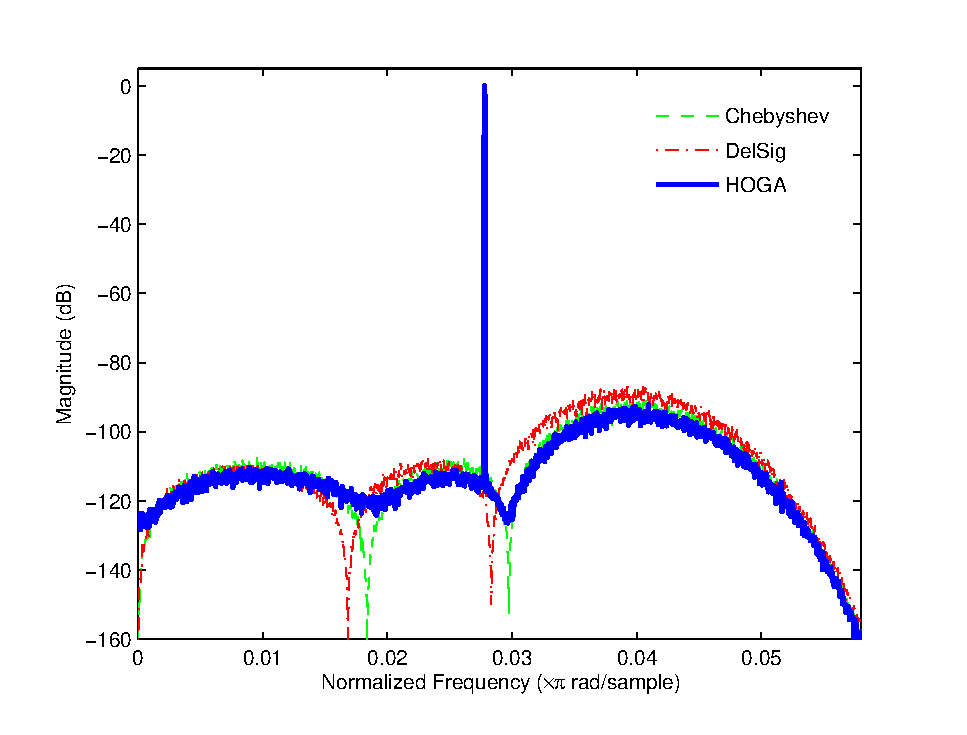
\includegraphics[width=0.75\textwidth]
{./matlab_figures/5th_order_spectra.eps}
	\captionsetup{justification=centering}
	\caption[]
{5th Order Output PSD Comparison\\
OSR: 32 - BW: $\pi$/OSR (rad/sample)- FFT Length: 8192}
	\label{fig:PSD_comparison_5}
\end{figure}
%----------------------- 
From the spectra shown in Figure \ref{fig:PSD_comparison_5}, the calculated SNRs and DRs
for the DelSig Toolbox, Chebyshev filter, and HOG algorithm based design method are
summarized in Table \ref{tbl:results_comparison_5}. Based on the SNR and DR values, it can
be seen that the HOG algorithm based design produces NTFs and STFs which achieve a higher
effective resolution than both the DelSig method and the Chebyshev filter.
%----------------------------
\begin{table}[htbp]
 \begin{center}
 \caption[5th Order \DS Modulator Results]{5th Order \DS Modulators: Calculated SNRs and
DRs}
 \label{tbl:results_comparison_5}
 \begin{tabular}{ l c c }\toprule
 \textbf{Design Method}  & \textbf{SNR$_\text{dB}$} & \textbf{DR$_\text{dB}$} \\ \midrule
        DelSig Toolbox   &     83       &     66      \\
        Chebyshev Filter &     81       &     72      \\
        HOG Algorithm    &     87       &     76      \\ \bottomrule
\end{tabular}
\end{center}
\end{table}
%----------------------------

Figure \ref{fig:NTF_comparison_6} shows a comparison of the NTF magnitude responses for
the various design techniques for a 6th order \DS modulator with an OSR of 32. Again, the
peak and average stopband spectrum for NTFs determined by the HOG algorithm is lower than
both the classical Chebyshev based NTF and the Delta Sigma toolbox's NTF and has a
stopband shape which reflects the optimization for a weighted combination of SNR and DR. 
%-----------------------
\begin{figure}[htbp]
	\centering
	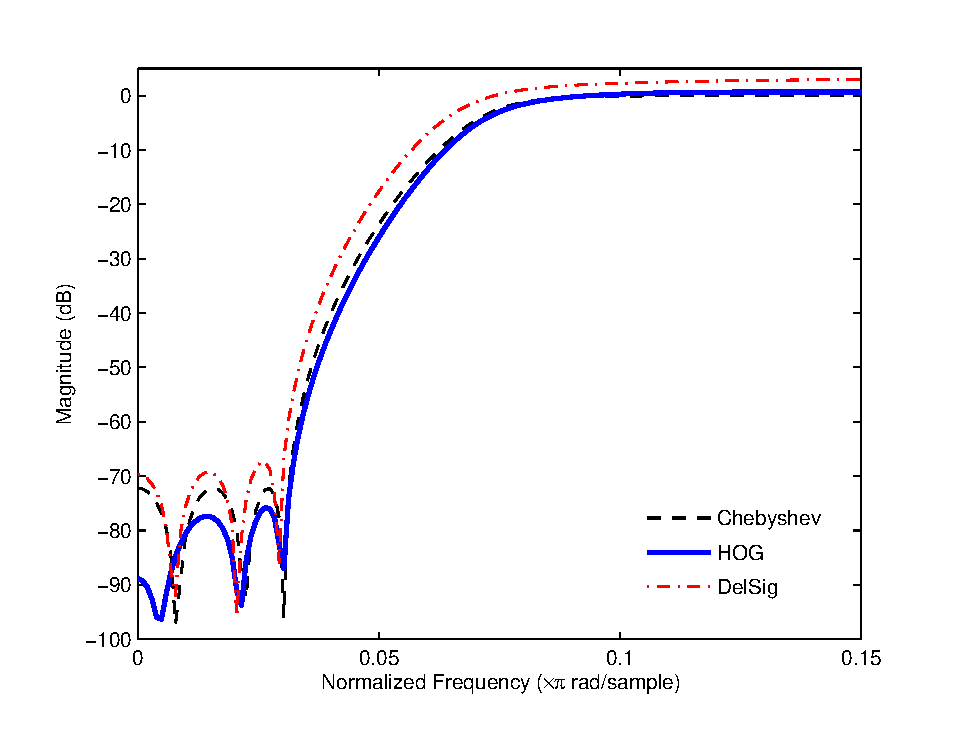
\includegraphics[width=0.75\textwidth]
{./matlab_figures/6th_order_NTFs.eps}
	\caption[]
{6th Order NTF Comparison\\
OSR: 32 - BW: $\pi$/OSR (rad/sample)}
	\label{fig:NTF_comparison_6}
\end{figure}
%-----------------------

Figure \ref{fig:STF_comparison_6} shows a comparison of the STF
magnitude responses for the corresponding NTFs  illustrated in Figure
\ref{fig:NTF_comparison_6}.
%-----------------------
\begin{figure}[htbp]
	\centering
	\includegraphics[width=0.75\textwidth]
{./matlab_figures/6th_order_STFs.eps}
	\caption[]
{6th Order STF Comparison\\
OSR: 32 - BW: $\pi$/OSR (rad/sample)}
	\label{fig:STF_comparison_6}
\end{figure}
%-----------------------
Again, the passband of the STF designed with the HOG algorithm, shown in Figure
\ref{fig:STF_comparison_6}, was optimized as described in Section
\ref{sec:STF_Objective_Function}.

Figure \ref{fig:PSD_comparison_6} illustrates the output spectra for the 6th order
\DS modulator that uses the STFs and NTFs shown in Figures \ref{fig:NTF_comparison_6} and
\ref{fig:STF_comparison_6}.
%-----------------------
\begin{figure}[htbp]
	\centering
	\includegraphics[width=0.75\textwidth]
{./matlab_figures/6th_order_spectra.eps}
	\captionsetup{justification=centering}
	\caption[]
{6th Order Output PSD Comparison\\
OSR: 32 - BW: $\pi$/OSR (rad/sample) - FFT Length: 8192}
	\label{fig:PSD_comparison_6}
\end{figure} 
%-----------------------
From the spectra shown in Figure \ref{fig:PSD_comparison_6}, the calculated SNRs and DRs
for the DelSig Toolbox, Chebyshev filter, and HOG algorithm based design method are
summarized in Table \ref{tbl:results_comparison_6}. Based on the SNR and DR values, it can
be seen that the HOG algorithm based design produces NTFs and STFs which achieve a higher
effective resolution than both the DelSig method and the Chebyshev filter.
%----------------------------
\begin{table}[htbp]
 \begin{center}
 \caption[6th Order \DS Modulator Results]{6th Order \DS Modulators: Calculated SNRs and
DRs}
 \label{tbl:results_comparison_6}
 \begin{tabular}{ l c c }\toprule
 \textbf{Design Method}  & \textbf{SNR$_\text{dB}$} & \textbf{DR$_\text{dB}$} \\ \midrule
        DelSig Toolbox   &     88       &     74      \\
        Chebyshev Filter &     87       &     77      \\
        HOG Algorithm    &     91       &     80      \\ \bottomrule
\end{tabular}
\end{center}
\end{table}
%----------------------------

Several \DS modulators were designed using the methods previously described. Figures
\ref{fig:SNR_DR_32_comparison}, \ref{fig:SNR_DR_64_comparison}, and
\ref{fig:SNR_DR_128_comparison} summarize the resulting SNRs and DRs as a function of
filter order for OSRs of 32, 64, and 128, respectively. Note that the HOG algorithm based
method provides improved SNR and DR over both the classical and contemporary design
methods.
%-----------------------
\begin{figure}[htbp]
	\centering
	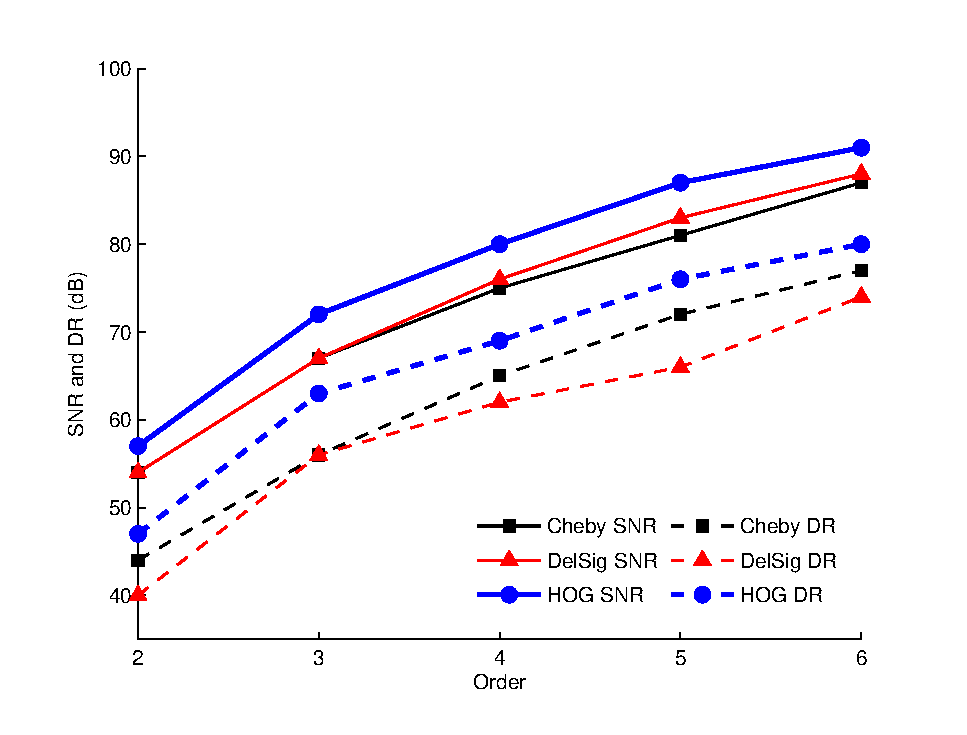
\includegraphics[width=0.75\textwidth]{./matlab_figures/OSR_32_chart.eps}
	\caption{SNR and DR Results with $\text{OSR}=32$}
	\label{fig:SNR_DR_32_comparison}
\end{figure}
%-----------------------
\begin{figure}[htbp]
	\centering
	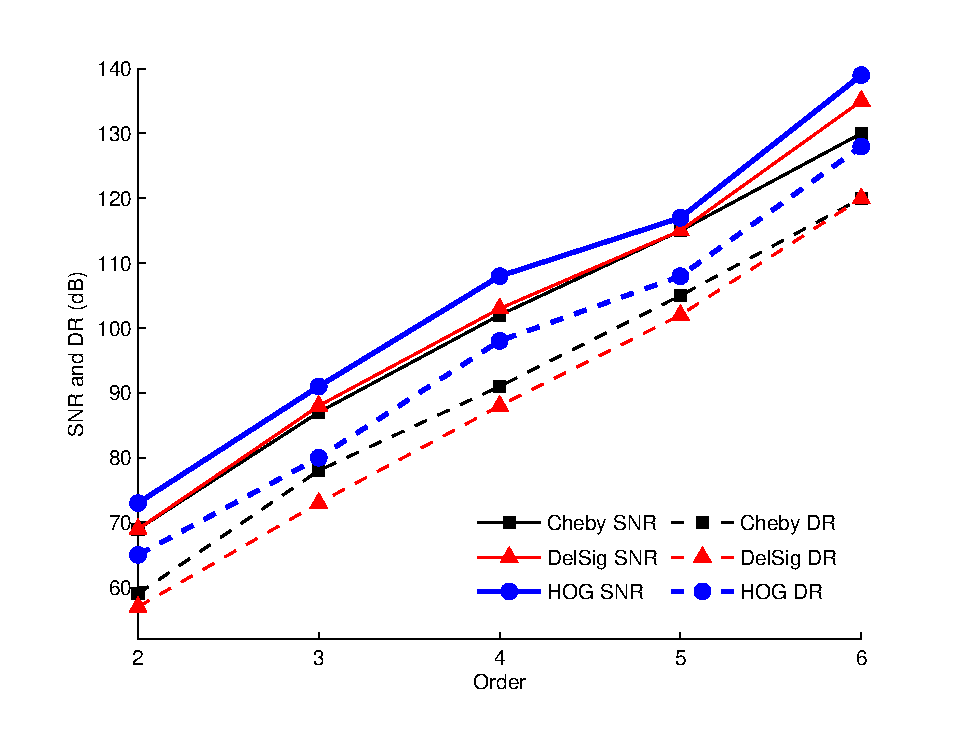
\includegraphics[width=0.75\textwidth]{./matlab_figures/OSR_64_chart.eps}
	\caption{SNR and DR Results with $\text{OSR}=64$}
	\label{fig:SNR_DR_64_comparison}
\end{figure}
%-----------------------
\begin{figure}[htbp]
	\centering
	\includegraphics[width=0.75\textwidth]{./matlab_figures/OSR_128_chart.eps}
	\caption{SNR and DR Results with $\text{OSR}=128$}
	\label{fig:SNR_DR_128_comparison}
\end{figure}
%-----------------------